\chap{Numbers and Displays}
\section{Introduction}
This is an exercise in designing combinational circuits that can perform binary-to-decimal number conversion and binary-coded-decimal (BCD) addition.\\
In previous parts, we design and implemented:
\begin{itemize}
    \item Two 7-segment displays inputed by the switches $SW_{7-0}$.
    \item Two-digit decimal represented by 7-segment displays,inputed by the switches $SW_{3-0}$(includes a comparator).
    \item full adder.
    \item Circuit that adds the two BCD digits.
\end{itemize}
\section{Part II}
\begin{itemize}
    \item [] \textbf{REQUIREMENT}
        \begin{enumerate}
            \item You are to design a circuit that converts a four-bit binary number $V = v_3v_2v_1v_0$ into its two-digit decimal equivalent $D = d_1d_0$. The table below shows the required output values. A partial design of this circuit is given in the figure below.
              \begin{figure}[h]
                \centering
                \hfill
                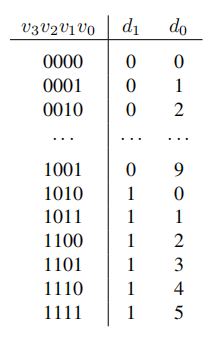
\includegraphics[width=4cm]{source/picture/Lab2/Lab2_table1.png}
                \hfill
                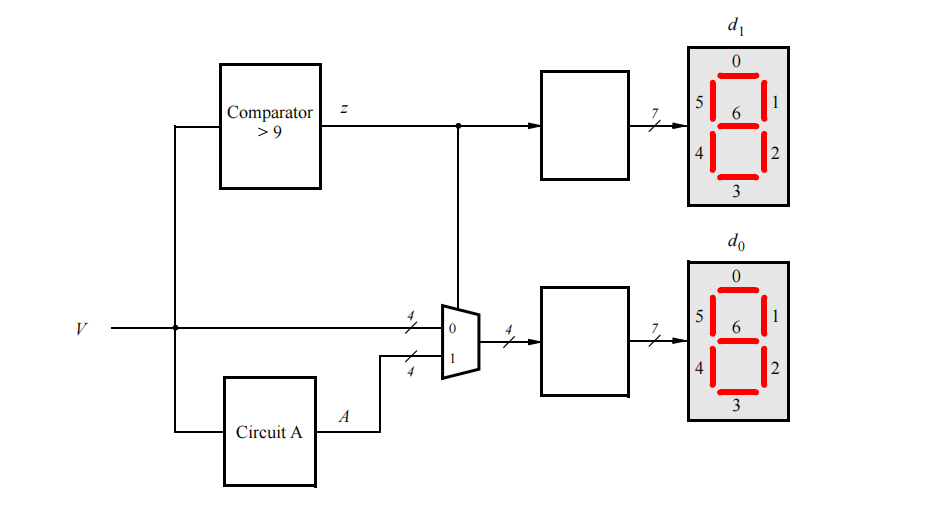
\includegraphics[width=10cm]{source/picture/Lab2/Lab2_figure1.png}
                \hfill
            \end{figure}
            \item  For the input values V ≤ 9, \textbf{the circuit A} does not matter, because the multiplexer in Figure above  just selects V in these cases. But for the input values V > 9, the multiplexer will select A.
        \end{enumerate}
    \item [] \textbf{SOLUTION}
        \begin{itemize}
            \item [] \textbf{Circuit A} is implemented using the hint of the requirement above.
                \begin{lstlisting}[language=verilog]
module circuitA(A_in, A_out);
	input		[3:0]A_in;
	output	[3:0]A_out;
	
	assign	A_out[3] = 0;
	assign 	A_out[2] = A_in[2]& A_in[1];
	assign	A_out[1] = A_in[2]&~A_in[1];
	assign 	A_out[0] = A_in[2]& A_in[0]  
					      +~A_in[2]&~A_in[0];
			
endmodule
                \end{lstlisting}
            \item [] \textbf{comparew9} indicate if the input greater than 9.
                \begin{lstlisting}[language=verilog]
module comparew9(com_in, com_out);
	input 	[3:0]com_in;
	output	com_out;
	assign 	com_out = com_in[3] & (com_in[2]|com_in[1]);
endmodule
                \end{lstlisting}
            \item [] \textbf{one\_to\_4btis} is used for translate the output of comparew9 block from 1 bits to 4 bits
                \begin{lstlisting}[language=verilog]
module multi_4bits(out, in0, in1, s);
	input		[3:0]in0,in1;
	input		s;
	output	[3:0]out;
	
	assign out = (in0&{4{~s}})|(in1&{4{s}}); 
endmodule
                \end{lstlisting}            
            \item [] \textbf{multi\_4bits} is user to choose the signal from \textbf{circuitA} and input, if input > 9, choose the result of block \textbf{circuitA.}
                \begin{lstlisting}[language=verilog]
module one_to_4bits(in,out);
	input		in;
	output	[3:0]out;
	assign 	out = (4'b0000) | in;
endmodule
                \end{lstlisting}               
            \item [] Finally, we wired these parts together. 
            \begin{figure}[h]
                \centering
                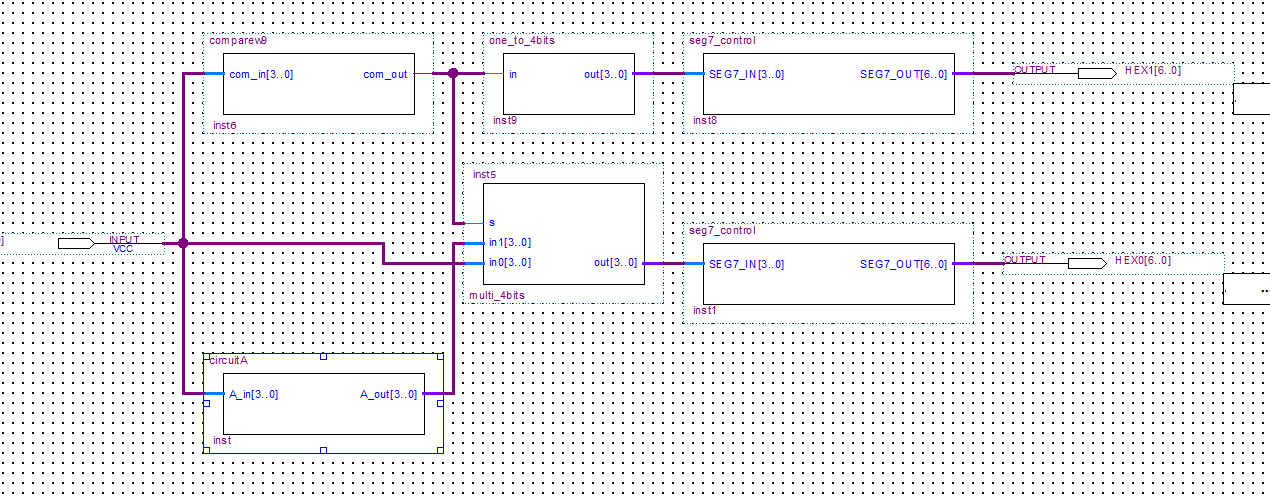
\includegraphics[width=\textwidth]{source/picture/Lab2/Lab2_2.png}
            \end{figure}
        \end{itemize}
\end{itemize}
\clearpage
\section{Part IV}
\begin{itemize}
    \item []\textbf{REQUIREMENT}
        \begin{enumerate}
            \item In part II we discussed the conversion of binary numbers into decimal digits. For this part you are to design a circuit that has two decimal digits, X and Y , as inputs. Each decimal digit is represented as a 4-bit number. In technical literature this is referred to as the binary coded decimal (BCD) representation.
            \item You are to design a circuit that adds the two BCD digits. The inputs to your circuit are the numbers X and Y , plus a carry-in, $c_{in}$. When these inputs are added, the result will be a 5-bit binary number. But this result is to be displayed on 7-segment displays as a two-digit BCD sum $S_1S_0$. 
        \end{enumerate}
    \item []\textbf{SOLUTION}
        \begin{itemize}
            \item []In this design, we use 2 block, namely: \textbf{sum4bits} and \textbf{display7SEG}.
                \begin{itemize}
                    \item []\textbf{Sum4bits} is the combination of 4 full-adder block.
                        \begin{lstlisting}[language=verilog]
module sum4bits(A,B,C_IN,SUM,C_OUT);
	input		[3:0]A,B;
	input		C_IN;
	output	[3:0]SUM;
	output	C_OUT;
	wire		C_1, C_2, C_3;
	full_adder inst1 (.a(A[0]), .b(B[0]), .c_i(C_IN),                      .s(SUM[0]), .c_o(C1));
	full_adder inst2 (.a(A[1]), .b(B[1]), .c_i(C1),                        .s(SUM[1]), .c_o(C2));
	full_adder inst3 (.a(A[2]), .b(B[2]), .c_i(C2),                        .s(SUM[2]), .c_o(C3));
	full_adder inst4 (.a(A[3]), .b(B[3]), .c_i(C3),                        .s(SUM[3]), .c_o(C_OUT));
endmodule
module full_adder(a,b,c_i,s,c_o);
	input 	a,b,c_i;
	output	s, c_o;
	assign 	s 		= c_i ^ (a^b);
	assign 	c_o	= (c_i & (a^b)) | (b & ~(a^b));
endmodule 
                        \end{lstlisting}
                    \item []\textbf{display7SEG}
                        \begin{lstlisting}[language=verilog]
module display7SEG(num, carry , hex0, hex1);
	input 	[3:0]num;
	input 	carry;
	output	[6:0]hex0, hex1;
	wire		[3:0]A_out;
	wire 		[3:0]num_plus6;
	wire		select;
	wire		com_out;
	wire		[3:0]seg7_1_in;
	wire		[3:0]seg7_0_in;
	circuitA 		inst0	(.A_in(num), .A_out(A_out));
	comparew9 		inst1	(.com_in(num),                                        .com_out(com_out));
	or select_char_1 		(select,carry,com_out);
	multi_4bits 	inst4	(.out(seg7_0_in), .in0(num),                          .in1(A_out), .s(select));
	one_to_4bits 	inst5	(.out(seg7_1_in),                                     .in(select));
	seg7_control 	inst6	(.SEG7_IN(seg7_0_in),                                 .SEG7_OUT(hex0));
	seg7_control 	inst7	(.SEG7_IN(seg7_1_in),                                 .SEG7_OUT(hex1));
endmodule
                        \end{lstlisting}
                    \item [] In \textbf{module part4}
                        \begin{lstlisting} [language=verilog]
module part4(X,Y,HEX0,HEX1);
	input 	[3:0]X,Y;
	output	[6:0]HEX0,HEX1;
	wire [3:0]num;
	wire carry;
	sum4bits 	inst0 (.A(X), .B(Y), .C_IN(0), .SUM(num), .C_OUT(carry));
	display7SEG	inst1 (.num(num), .carry(carry), .hex0(HEX0), .hex1(HEX1));
endmodule
                        \end{lstlisting}
                \end{itemize} This is our design
                    \begin{figure}[h]
                        \centering
                        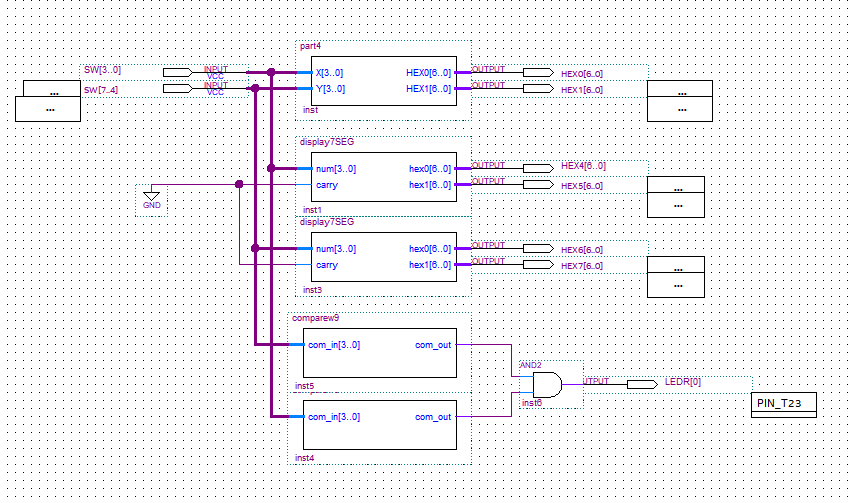
\includegraphics[width=\textwidth]{source/picture/Lab2/Lab2_4.png}
                    \end{figure}
        \end{itemize}
    
\end{itemize}
\clearpage